% Created 2024-09-01 Sun 12:06
% Intended LaTeX compiler: pdflatex
\documentclass[11pt]{article}
\usepackage[utf8]{inputenc}
\usepackage[T1]{fontenc}
\usepackage{graphicx}
\usepackage{longtable}
\usepackage{wrapfig}
\usepackage{rotating}
\usepackage[normalem]{ulem}
\usepackage{amsmath}
\usepackage{amssymb}
\usepackage{capt-of}
\usepackage{hyperref}
\usepackage{minted}
\usepackage{xcolor}
\usepackage{hyperref}
\usepackage{tocloft}
\usepackage[margin=1.8cm]{geometry}
\usepackage{fancyheadings}
\usepackage{minted}
\usepackage[utf8]{inputenc}
\usepackage{amsmath}
\usepackage{amsfonts}
\usepackage{amssymb}
\usepackage{titlesec}
\usemintedstyle{manni}
\usepackage{enumitem}
\usepackage{pdfpages}
\setlength{\parindent}{0cm}
\usepackage{parskip}
\usemintedstyle{friendly}
\usepackage{graphicx}
\usepackage{listings}
\usepackage{float}
\usepackage{colortbl}
\usepackage{booktabs}
\usepackage{wrapfig}
\usepackage{tabularx}
\usepackage{color}
\usepackage{tabularray}
\restylefloat{table}
\usemintedstyle{dracula}
\usepackage[table]{xcolor}
\usepackage{setspace}
\usepackage[none]{hyphenat}
\usepackage{xcolor}
\usepackage{pagecolor}
\definecolor{solarizedBase03}{RGB}{0, 43, 54}
\definecolor{solarizedBase02}{RGB}{7, 54, 66}
\definecolor{solarizedBase01}{RGB}{88, 110, 117}
\definecolor{solarizedBase00}{RGB}{101, 123, 131}
\definecolor{solarizedBase0}{RGB}{131, 148, 150}
\definecolor{solarizedBase1}{RGB}{147, 161, 161}
\definecolor{solarizedBase2}{RGB}{238, 232, 213}
\definecolor{solarizedBase3}{RGB}{253, 246, 227}
\definecolor{solarizedYellow}{RGB}{181, 137, 0}
\definecolor{solarizedOrange}{RGB}{203, 75, 22}
\definecolor{solarizedRed}{RGB}{220, 50, 47}
\definecolor{solarizedMagenta}{RGB}{211, 54, 130}
\definecolor{solarizedViolet}{RGB}{108, 113, 196}
\definecolor{solarizedBlue}{RGB}{38, 139, 210}
\definecolor{solarizedCyan}{RGB}{42, 161, 152}
\definecolor{solarizedGreen}{RGB}{133, 153, 0}
\pagecolor{solarizedBase3}
\color{solarizedBase00}
\hypersetup{
colorlinks=true,
linkcolor=solarizedBlue,
filecolor=solarizedGreen,
urlcolor=solarizedOrange,
citecolor=solarizedMagenta,
}
\titleformat{\section}
{\color{solarizedBlue}\normalfont\Large\bfseries}
{\color{solarizedBlue}\thesection}{1em}{}
\titleformat{\subsection}
{\color{solarizedGreen}\normalfont\large\bfseries}
{\color{solarizedGreen}\thesubsection}{1em}{}
\titleformat{\subsubsection}
{\color{solarizedYellow}\normalfont\normalsize\bfseries}
{\color{solarizedYellow}\thesubsubsection}{1em}{}
\definecolor{draculaBackground}{HTML}{282a36}
\definecolor{draculaForeground}{HTML}{f8f8f2}
\definecolor{draculaSelection}{HTML}{44475a}
\definecolor{draculaComment}{HTML}{6272a4}
\definecolor{draculaCyan}{HTML}{8be9fd}
\definecolor{draculaGreen}{HTML}{50fa7b}
\definecolor{draculaOrange}{HTML}{ffb86c}
\definecolor{draculaPink}{HTML}{ff79c6}
\definecolor{draculaPurple}{HTML}{bd93f9}
\definecolor{draculaRed}{HTML}{ff5555}
\definecolor{draculaYellow}{HTML}{f1fa8c}
\usepackage[table,xcdraw]{xcolor}
\author{Robert Alicea}
\date{\today}
\title{P.S. 192 Family Handbook 2023-24}
\hypersetup{
 pdfauthor={Robert Alicea},
 pdftitle={P.S. 192 Family Handbook 2023-24},
 pdfkeywords={},
 pdfsubject={},
 pdfcreator={Emacs 29.4 (Org mode 9.6.15)}, 
 pdflang={English}}
\begin{document}

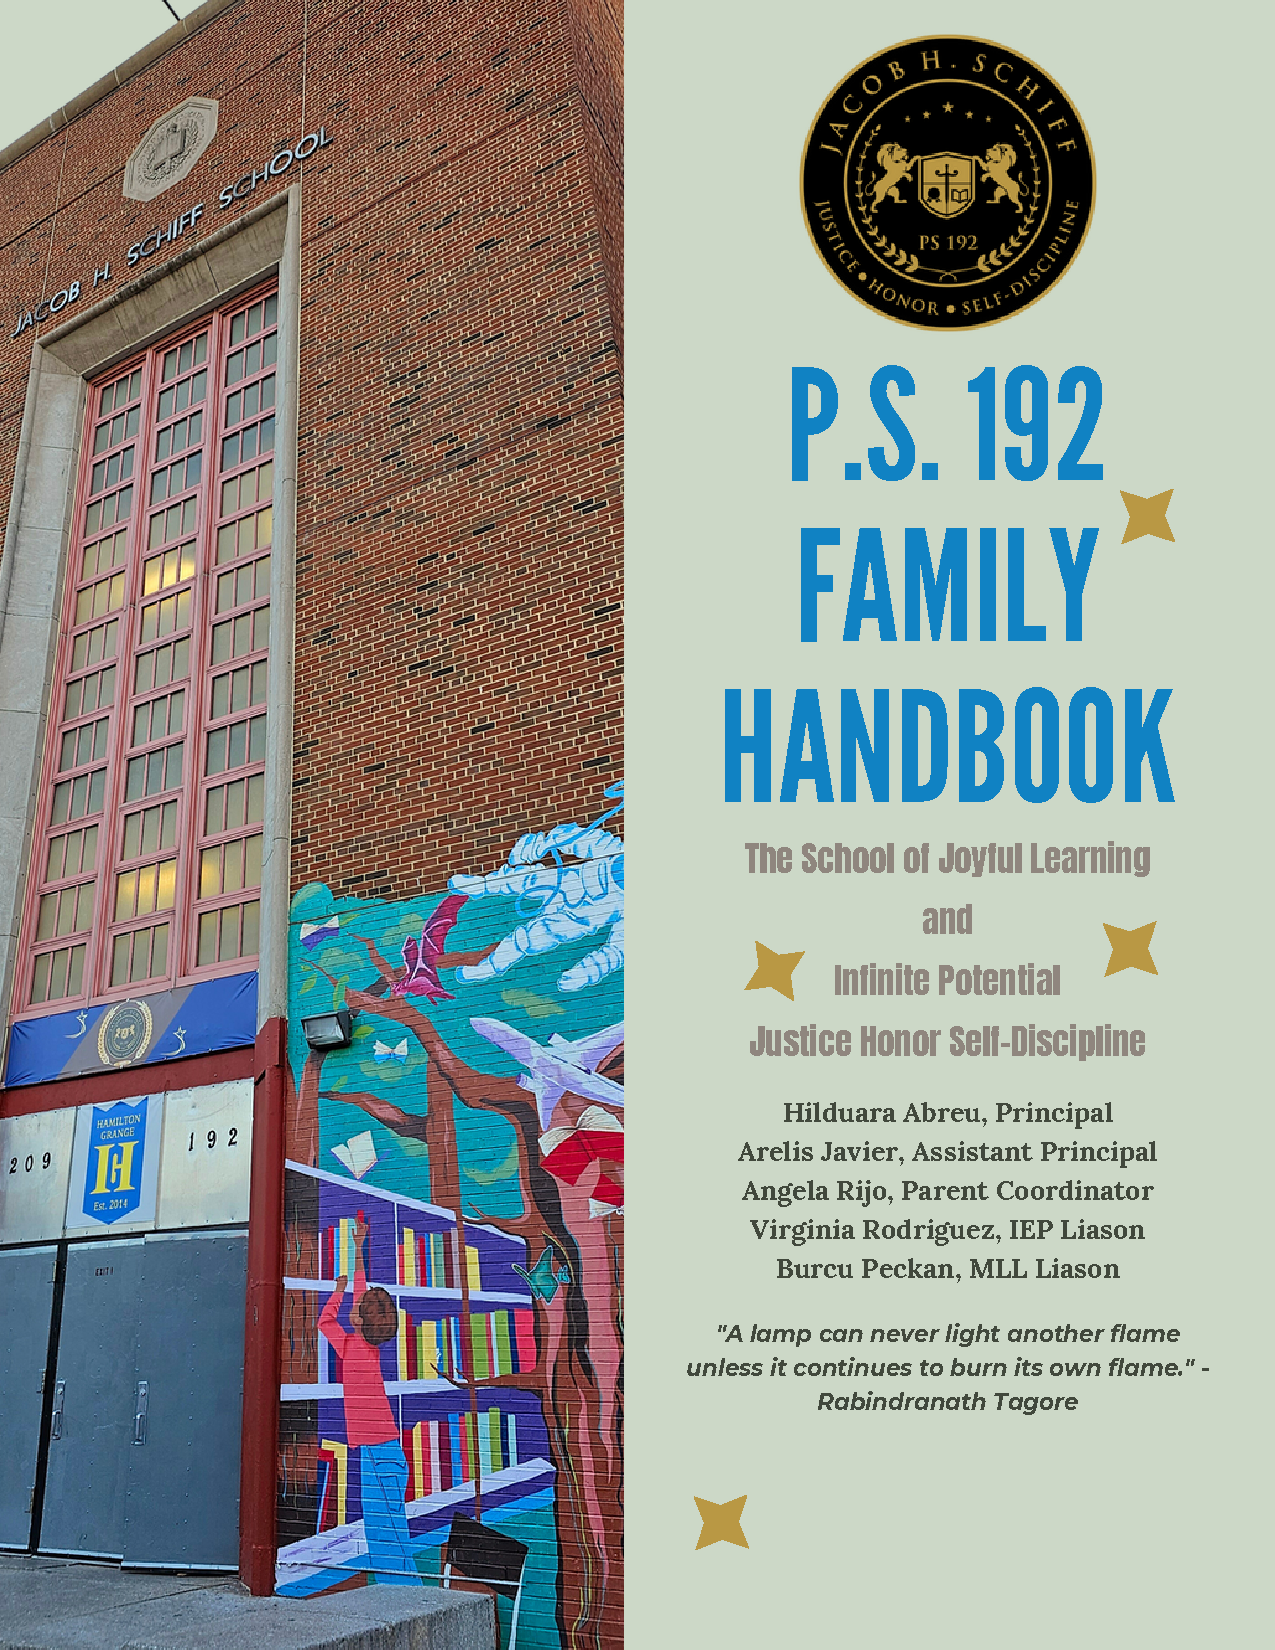
\includepdf[pages=1,fitpaper]{pdf.pdf}

\pagenumbering{\fancyhf{}}
\pagestyle{headings}
\pagenumbering{arabic}

\fancyhead[R]{\thepage}

\fancyfoot[C]{The School of joyful Learning \& Infinite Potential}
\pagestyle{fancy}
\renewcommand{\footrulewidth}{1px}

\definecolor{dkgreen}{rgb}{0,0.6,0}
\definecolor{gray}{rgb}{0.5,0.5,0.5}
\definecolor{mauve}{rgb}{0.58,0,0.82}

\clearpage
\clearpage \tableofcontents \clearpage


\section{About the Family Handbook}
\label{sec:orgd22e1a0}
The Family Handbook is an essential resource for understanding PS 192's policies and procedures, which are meticulously designed to foster a positive, educationally-focused learning environment where our students thrive and grow. Recognizing that families are our students' first teachers, we aim to make you feel welcome and ensure full transparency regarding our educational approach and the structures that support it.

This handbook reflects the collective input of parents, students, and staff, dedicated to managing our inclusive community while prioritizing safety and equity. As a living document, it may evolve throughout the year to better serve our community's needs. Our team will reference this handbook to address your questions and concerns, reinforcing our commitment to a collaborative and supportive PS 192 community.

\clearpage

\section{Message from the Principal}
\label{sec:org4b673a2}

Welcome to P.S. 192, where excellence in education is not just a goal, but a way of life. It is with immense pleasure and pride that I extend my warmest greetings to you all as we embark on yet another exciting academic year.

At P.S. 192, we are more than just an educational institution; we are a community united by a shared vision of nurturing young minds and shaping future leaders. Our school’s emblem, proudly displaying the noble lion and lioness, symbolizes the strength, courage, and unwavering determination that define our journey together.

As we journey forward, we remain steadfast in our commitment to instill three core values into the hearts of our students: Justice, Honor, and Self-Discipline. These values are the guiding principles that underpin everything we do. They form the bedrock upon which we build character, foster empathy, and cultivate the leaders of tomorrow.

In the pages of this Family Handbook, you will find a wealth of information about our school’s policies, programs, and opportunities. It is designed to be your compass, helping you navigate the rich and rewarding educational experience we offer.

Together, as a united educational family, we will empower your child to explore their potential, embrace challenges, and emerge as confident, compassionate, and responsible individuals ready to make a positive impact on the world.

Thank you for entrusting us with the privilege of shaping your child’s future. Together, we will roar with pride as our students become the lions and lionesses of tomorrow, embodying the values of justice, honor, and self-discipline.

Respectfully yours,


\includegraphics[width=100px]{/var/home/rob/Documents/org-mode/ps192/ps192_family_handbook/hil_signature.png}

\textbf{\textbf{Hilduara Abreu, Principal}}

\textbf{\textbf{The School of Joyful Learning!}}

\href{https://www.ps192.org}{www.ps192.org}

\begin{figure}[b]  % The 'b' option places the figure at the bottom of the page
  \centering
  
\includegraphics[width=0.48\textwidth]{/var/home/rob/Documents/org-mode/ps192/ps192_family_handbook/1.png}
  \label{fig:fronpage bottom_image}
\end{figure}

\clearpage

\section{About P.S. 192}
\label{sec:org6f0a755}

Welcome to P.S. 192 | Jacob H. Schiff School, where we believe in nurturing "Infinite Potential" in every child. Our school is more than just a place of learning; it’s a community dedicated to unlocking the limitless abilities and intelligence within each of our students through dedication, learning, and resilience. We are committed to instilling core values of justice, honor, and self-discipline in every aspect of our educational journey.

\href{https://4.files.edl.io/760e/02/07/24/000734-b96f6af6-0f19-4829-999f-2eb23313280d.pdf}{PARENT NOTIFICATION LETTER FOR SCHOOLS DESIGNATED FOR LSI}

\subsection{History}
\label{sec:org07a03aa}

Our school was established in 1952, was once home to the Hebrew Orphan Asylum of New York (HOA). It began as a modest educational institution serving the local community.

Jacob H. Schiff’s contributions extended beyond our school, as he actively supported various initiatives that aimed to uplift marginalized communities, promote civil rights, and advance educational opportunities. His commitment to justice and social equity has left an enduring impact on our institution and our community.

\begin{figure}[htbp]
\centering

\includegraphics[width=1\textwidth]{/var/home/rob/Documents/org-mode/ps192/ps192_family_handbook/images/2.png}
\caption{School Motto "Good, better, best. Never let it rest until your good is better, and your better is best." St. Jerome}
\end{figure}

\subsection{Our Commitment}
\label{sec:orgfc95ce5}

We provide a dynamic learning environment with personalized support to each student, fostering curiosity, creativity, and critical thinking.

\subsection{Core Values}
\label{sec:org449705b}

\begin{itemize}
\item \textbf{\textbf{Justice:}} Teaching fairness and equity.
\item \textbf{\textbf{Honor:}} Emphasizing integrity and respect.
\item \textbf{\textbf{Self-Discipline:}} Guiding students to develop strong work ethics.
\end{itemize}

\subsection{Infinite Potential}
\label{sec:org9e72bd7}

We believe every child has boundless possibilities. By nurturing their potential and instilling core values, we prepare them for academic, social, and moral success.

\begin{figure}[htbp]
\centering

\includegraphics[width=1\textwidth]{/var/home/rob/Documents/org-mode/ps192/ps192_family_handbook/images/3.png}
\caption{Infinite Potential is the guiding star of our school, illuminating a path where students are emboldened to dream without boundaries and pursue a voyage of continuous learning and self-improvement. It is here, within the nurturing halls of PS192, that we ignite the spark of curiosity and fan the flames of possibility, forging a future replete with endless opportunities for each and every child.}
\end{figure}

\subsection{Mission}
\label{sec:orgf4bbf46}
To provide a welcoming, safe, resourceful, and nurturing environment that supports our school community's academic and social-emotional development where children are respected and engaged in challenging curricula that motivate them to realize their potential as active, lifelong learners. Through our guiding core values of Justice, Honor, and Self-discipline, we aspire to promote perseverance, love, empathy, and respect for oneself and others.

\href{https://4.files.edl.io/d109/09/17/23/012751-34dac161-8e19-4033-8c6b-f369007cab02.pdf}{The Home \& School Agreement}

\subsection{Vision}
\label{sec:org0389967}
To ensure all students acquire the essential knowledge and skills they need to become independent thinkers and become active participants and contributors in their roles as students and as members of society.

\subsection{School Motto}
\label{sec:org6bc67e9}

"Good, better, best. Never let it rest until your good is better, and your better is best."

\subsection{School-Wide Norms of Conduct}
\label{sec:org4d67c8b}
Daily recitation of the \href{https://www.ps192.org/apps/pages/index.jsp?uREC\_ID=1504973\&type=d\&pREC\_ID=2371090}{Positivity Pledge} promotes a positive and inclusive environment.

\subsection{Our Teaching Staff}
\label{sec:orgd89f40e}
Jacob H. Schiff PS 192 is distinguished by the exceptional quality of our teaching staff. Our educators are a diverse group, each bringing a wealth of skills and expertise to our school community. Collaboration among our teachers is paramount, as they share their talents and strengths to enhance learning and create abundant opportunities for our students.

Our faculty comprises 12 classroom teachers, a physical education instructor, an ENL teacher, and special education support staff. Additionally, we are proud to have two arts educators specializing in Drama and Music. We also engage consultants to offer specialized instruction in Dance and Visual Arts. Our dedicated Guidance Counselor and Social Worker are integral to fostering our students' social and emotional growth. We frequently welcome student teachers from prestigious institutions such as Bank Street College of Education and Columbia University's Teachers College. Complementing our faculty is a dedicated team of paraprofessionals who collaborate with our teachers and specialists to provide individualized support, ensuring every student's needs are met.

\section{Communication from P.S. 192 – Jacob H. Schiff}
\label{sec:org98e6b02}

At P.S. 192, we prioritize clear and consistent communication with our families to ensure everyone is informed and engaged. By primarily using electronic methods, we support environmental sustainability and facilitate translation for our diverse community.

Our communication methods include:
\begin{itemize}
\item \textbf{\textbf{Monthly Newsletter}}: Sent to parents email who are enrolled on our newsletter club in the \href{https://www.ps192.org}{website}.
\item \textbf{\textbf{ClassDojo}}: This platform includes a news feed for reminders and school highlights, as well as parent-to-teacher and parent-to-principal messaging, with built-in translation features.
\item \textbf{\textbf{Electronic Surveys}}: To gather feedback and improve our school community.
\item \textbf{\textbf{School Calendar}}: Stay updated with school events and important dates. \href{https://www.ps192.org/apps/events/}{School Calendar Link}
\item \textbf{\textbf{Website}}: Visit us at \href{https:www.ps192.org}{www.ps192.org} for comprehensive information and updates.
\item \textbf{\textbf{Others}}: robot calls, parent coordinator, regular mail, teachers, etc.
\end{itemize}

Through these channels, we aim to keep our P.S. 192 community well-informed and connected, supporting our shared goal of fostering a thriving educational environment for our students.

\section{Loopping Model \& Curricula}
\label{sec:org1db291d}

\subsection{Looping Model}
\label{sec:org6d89431}
Looping allows teachers to stay with the same group of students for more than one year, fostering strong relationships and a stable learning environment. This practice offers several benefits:
\begin{itemize}
\item \textbf{\textbf{Strong Teacher-Student Relationships:}} Teachers understand each child’s unique learning style, strengths, and areas of improvement, resulting in a more tailored educational experience.
\item \textbf{\textbf{Consistency and Stability:}} A familiar classroom environment reduces anxiety and encourages active participation.
\item \textbf{\textbf{Seamless Transition:}} Minimizes disruptions and ensures a smoother academic journey as students remain with a familiar teacher.
\item \textbf{\textbf{Academic Growth:}} Teachers build on the knowledge gained in the previous year, leading to improved academic outcomes.
\item \textbf{\textbf{Personalized Support:}} With a deeper understanding of each student’s needs, teachers can provide targeted interventions and support.
\end{itemize}

\subsection{Curricula}
\label{sec:org3cdc620}
We use a variety of curricula to provide a rich educational experience:
\begin{itemize}
\item \textbf{\textbf{Expeditionary Learning:}} Focuses on real-world learning, critical thinking, and problem-solving through hands-on activities and projects.
\item \textbf{\textbf{enVision Mathematics:}} Emphasizes a deep conceptual understanding of mathematics through visual models and personalized instruction.
\item \textbf{\textbf{Passport-to-Social-Studies:}} Encourages historical thinking, critical analysis, and the exploration of multiple perspectives.
\item \textbf{\textbf{Amplify Science:}} Students engage in scientific inquiry and engineering practices through interactive activities and digital simulations.
\item \textbf{\textbf{Sanford Harmony:}} A socio-emotional program that fosters positive classroom relationships and reduces disruptive behavior.
\end{itemize}

\href{https://4.files.edl.io/64e1/10/24/23/162457-5c04bb98-4658-4c66-b8c1-f3f1eee37250.pdf}{Promotional Criteria and Grading Policy 2023-24}

\subsection{Response to Intervention (RTI)}
\label{sec:orga2b6fea}

Our RTI framework ensures all students receive the support they need to reach their full potential. It includes:
\begin{itemize}
\item \textbf{\textbf{Tiered Instruction:}} Provides different levels of support based on student needs.
\item \textbf{\textbf{Progress Monitoring:}} Regularly assesses student progress to inform instruction.
\item \textbf{\textbf{Data-Driven Decision Making:}} Uses data to identify students who need additional support and to guide interventions.
\end{itemize}

\section{Assessment of Student Work}
\label{sec:org2b594b7}

\subsection{Reporting Student Progress}
\label{sec:org5583f1a}
Our grading policy includes:
\begin{itemize}
\item \textbf{\textbf{Homework Policy:}} Homework serves as a tool for developing good habits, reinforcing learning, and fostering family involvement. Assignments are meaningful, tailored to individual needs, and provide feedback.
\item \textbf{\textbf{Parental Involvement in Homework:}} Encourages parents to assist their child while fostering independence. Parents should communicate with teachers if their child struggles with homework.
\end{itemize}

\subsection{Standardized Testing}
\label{sec:org83bc805}
We conduct annual State assessments in compliance with federal and state directives. Families have the right to opt out of testing, and students who do not participate will engage in meaningful educational activities. These assessments are a key component of our educational program, designed to gauge student progress and identify areas for improvement.
\subsubsection{Types of Assessments:}
\label{sec:org3f16600}
\begin{itemize}
\item NY State Grades 3-8 English Language Arts (ELA) and Mathematics Tests: These exams are administered annually to students in grades 3 through 8. The ELA test assesses reading, writing, and language skills, while the Mathematics test evaluates problem-solving, computation, and mathematical reasoning.
\item NY State Science Test: This assessment is given to students in grades 4 and 8 to measure their understanding of core scientific concepts and their ability to apply scientific principles.
\item NYC Performance Tasks: In addition to state tests, students may participate in NYC performance tasks designed to assess critical thinking, problem-solving, and application of knowledge in real-world scenarios.
\end{itemize}

\section{Key Details for Families}
\label{sec:org6c62925}
\subsection{Meal Application Form}
\label{sec:org8755f20}
Breakfast, lunch, and after school meals are free for all New York City public school students. Although students no longer need to apply to receive free meals, we do encourage families to complete the online \href{https://www.opt-osfns.org/osfns/Resources/SchoolMealsApplicationOrderingSystem/Home.aspx}{Family Income Inquiry form} so that your school(s) can receive funding for the program. More information in \href{https://www.schools.nyc.gov/school-life/food/school-meals/food-service-for-parents-and-students}{NYC DOE Website}

\subsection{Attendance and Lateness}
\label{sec:org7606b9a}
Consistent attendance plays a pivotal role in achieving success within our educational institution. Each instance of absence equates to a forfeiture of valuable instructional time and poses a potential risk to your child’s academic progress, potentially causing them to lag behind in the acquisition of fundamental skills. See \href{https://4.files.edl.io/3b80/09/17/23/025447-0ea48bb2-237d-4b10-bb0c-c54719f66e99.pdf}{Bell Schedule Document}.

It is imperative to acknowledge that your child’s attendance, encompassing punctuality as well, is meticulously documented as part of their permanent educational dossier. This attendance record is meticulously maintained within the Automated Schools (ATS), a real-time student data tracking system sanctioned by the New York City Department of Education (NYC DOE). The vigilance with which we monitor attendance underscores its significance, not only as an individual indicator but also as a substantial component contributing to the evaluation of our school’s overall performance by the NYC DOE, which, in turn, holds us accountable to the highest educational standards. Please be aware that in the event of excessive absences, the ATS system will automatically trigger the generation of a Form 407 Attendance Follow-up and Outreach Referral, followed by a scheduled home visit as a proactive measure.

For a more comprehensive understanding of our school’s attendance policies and procedures, we invite you to consult the attached P.S. 192 Attendance Policy, which provides detailed information on this crucial aspect of your child’s education. Your partnership in ensuring regular attendance is greatly appreciated, as it significantly contributes to your child’s educational journey. Should you have any inquiries or require further clarification, please do not hesitate to reach out to Principal Abreu. Together, we can provide the best educational experience for your child.See \hyperref[sec:orge2fd45a]{Attendance and Latenes}

\subsubsection{Arrival}
\label{sec:orgf184a10}
Our school commences its instructional day promptly at 8:00 AM, concluding at 2:20 PM. We kindly request your cooperation in ensuring your child’s timely arrival at the beginning and prompt pickup at the end of the school day. Our dedicated school staff diligently uphold the safety and accountability of all children under their care at all times. It is of utmost importance that every family adheres to our established protocols for both drop-off and dismissal, as this is essential for us to maintain this high standard of safety. For further guidance on attendance and punctuality, please refer to the section below outlining the Department of Education’s policies. Additionally, we have included an attached appendix on Attendance that provides comprehensive information regarding arrival, dismissal, and overall attendance procedures.
\begin{itemize}
\item \textbf{\textbf{Arrival:}} Students can be dropped off at 8:00 AM for regular arrival or at 7:40 AM if they are having school breakfast.
\item \textbf{\textbf{Late Arrivals:}} Tardiness is recorded in the ATS system. Email notifications are sent for late arrivals at \href{mailto:arijo@schools.nyc.gov}{arijo@schools.nyc.gov}.
\item \textbf{\textbf{Dismissal:}} Students are picked up at 2:20 PM. Only authorized adults can pick up students.
\end{itemize}

\subsubsection{Late Arrival}
\label{sec:org5a77de5}
We kindly request your punctuality, as tardiness can disrupt the day to day operation of the school and potentially impact a child’s educational progress. Each morning, our classes commence with a brief morning meeting followed by instructional activities. In the event that your child arrives late, the teacher will promptly inform the main office, where the tardiness is recorded in the ATS system. Should your child arrive after the designated attendance submission time, typically around 8:30 am, you may receive an email notification from the Department of Education (DOE) indicating their absence. This occurs because all attendance records must be finalized by a specific time, and any changes made after this deadline will not be reflected in the system until the following morning. Your cooperation in ensuring timely arrivals is greatly appreciated. Students should not miss school except in the case of illness. Please send a note to scuesta@schools.nyc.gov EACH time your child is absent. A doctor’s note is required after two (2) days. We strongly advise families to not schedule vacations when school is in session. We also request that every effort be made to schedule a doctor’s appointments after school hours. If this is not possible, please have your child attend for part of the day.

\subsubsection{Dismissal}
\label{sec:org2940aa0}
Dismissal is at 2:20 PM Students are picked up outside inside the school yard. Please be prompt to pick up your child. Late pickups cause your child unnecessary anxiety, inconvenience teachers and jeopardize our ability to keep a safe school environment.

We can only release your child to adults designated on the emergency contact card or on the \href{https://www.schoolsaccount.nyc/}{NYCSA} Parent Account. This applies even if it is another P.S. 192 family you are asking to pick up your child. If a teacher is not familiar with the person picking up, they may ask for ID to ensure that the person is on the list.

Dismissal is not a time for a long conversation with staff. Staff must remain focused on the safety of all their students. If you need to speak with a staff member, please schedule a time to do so. You may send an email or a ClassDojo text to the child’s teacher.

Please make every effort to be on time for pick up - staff have families to go home to or other work assignments. If you think you will be late for dismissal please call the main office to notify us as soon as possible so we can inform your child and relevant staff and so that we can plan for staff to stay with students if needed. Students who are still in their classroom or the yard 10 minutes after dismissal are taken to the main office and parents/guardians are called.

At the beginning of the year, you must fill out a dismissal form listing who will pick up your child each day. We also ask for their contact information in case they are late. Please make sure to update this form with the office if there are long term changes like new babysitters, after school programs, classes or clubs.

If there is a change to this dismissal information for the day, you must email Ms. Rijo at arijo@schools.nyc.gov before 11 AM the day of the change. (8 AM for half days.) This allows us enough time to make everyone involved in dismissal knows. Please do NOT communicate dismissal changes to teachers as they are not able to view their email during the school day.

Please plan ahead regarding changes in your pick up procedure. Frequent changes to dismissal plans can be unsettling to your child and disruptive to the class and school.

\subsubsection{Early Dismissal}
\label{sec:org462786b}
If you are picking up your child please email us ahead of time at arijo@schools.nyc.gov. When you arrive, a staff member will bring your child to you and have you sign the early pick up book. Only authorized adults may sign out a student. Even if your student is an independent walker, they must be picked up by an adult if they are leaving before the end of the school day. Early dismissal MUST be before 1:30 PM. If you are not here before 2:00 PM you must wait until regular dismissal at 2:20 PM.
\subsection{Transportation}
\label{sec:orgd2d8913}
In accordance with Chancellor’s Regulation A-801 (see below for regulation with translations) , the DOE provides transportation to all eligible New York City students in public, charter, and non-public schools. In partnership with the Metropolitan Transit Authority (MTA) and our \href{https://www.schools.nyc.gov/school-life/transportation/bus-companies-for-school-age-children}{school age} and \href{https://www.schools.nyc.gov/school-life/transportation/pre-k-and-early-intervention-bus-companies}{preschool} bus companies, our mission is to ensure safe and reliable transportation to and from school.

See \href{https://www.schools.nyc.gov/school-life/transportation/transportation-rights}{Transportation Rights} for what you and your child can expect from DOE transportation services.

See \href{https://www.schools.nyc.gov/school-life/transportation/transportation-guide}{Transportation Guide} (Open external link) for a summarized introduction to transportation options, eligibility, and more.

Contact our Parent Coordinator for eligibility details regarding school bus or metro card services. More info \hyperref[sec:org9f1b2f3]{Apendix B: Transportation Eligibility}

\subsection{Wellness and Healthy Eating}
\label{sec:orgd9c14fc}
The New York City Department of Education (NYC DOE) is dedicated to collaborating with schools, families, and the community to ensure students graduate equipped to care for their minds, bodies, and those around them. We foster supportive and health-promoting learning environments that are inclusive and reflect the city's rich diversity, benefiting all students. Evidence indicates that good nutrition and physical activity are strongly linked to positive academic outcomes, and we actively promote these through various programs like the USDA's School Breakfast Program. As participants in the National School Lunch and Breakfast Programs, we adhere to a local wellness policy that supports student health and addresses childhood obesity. Our Citywide Wellness Policy ensures students receive quality physical and health education, access to healthy foods, and opportunities for physical activity, all within environments that minimize commercial distractions and encourage lifelong healthy behaviors.

We promote \href{https://infohub.nyced.org/in-our-schools/policies/doe-wellness-policy}{healthy lifestyles} through education on nutrition and physical fitness.

\subsection{Nutritional Guidelines and Policies at PS 192}
\label{sec:org590e308}
Ensuring that our students start the day with a nutritious breakfast is vital for their success and well-being at school. Breakfast is provided free of charge to all students and is available beginning at 7:40 a.m.

Our lunch and recess period commences at 10: a.m. Like breakfast, school lunch is also free for all students. While students are welcome to bring lunch from home, please be advised that no refrigeration is available for these lunches.

\subsubsection{Allergy and Nutrition Policies:}
\label{sec:orgb38dcf1}
\begin{itemize}
\item \textbf{\textbf{No Nuts Policy:}} We have several students with severe nut allergies. To safeguard their health and safety, PS 192 enforces a strict no-nuts policy for all lunches and snacks.
\item \textbf{\textbf{Healthy Food Policy:}} We prioritize the health and nutritional well-being of our students. Therefore, we ask that you do not send candy, chips, cookies, or sugary drinks with your child. Additionally, gum chewing is not permitted unless arranged with a classroom teacher for sensory needs.
\end{itemize}

\subsubsection{Menus and Snack Guidelines:}
\label{sec:orgf3e14c1}
The menus for school breakfast and lunch can be found on the DOE website: \href{https://www.schools.nyc.gov/school-life/food/menus}{NYC DOE Food Menus}.

Due to our late lunch schedule, we have a daily snack time. Snacks are generously donated by our families. At the start of the school year, your classroom teacher or class parent will organize a schedule and invite you to sign up to provide snacks for the class for one week. If your family is unable to contribute for any reason, please inform us.

We aim for our snacks to support healthy dietary habits. Therefore, please provide healthy, nut-free snacks in individual portions. Your classroom teacher or class parent will inform you of any additional allergies to consider when contributing snacks.

Thank you for your cooperation in adhering to these guidelines and for your ongoing support in promoting a healthy and safe environment for all our students.
Breakfast and lunch are free for all students. Please avoid sending nuts and junk food.

\subsection{Recess}
\label{sec:org441bac8}
All students at Jacob H. Schiff PS 192 enjoy a supervised recess period, which is scheduled either before or after lunch. For our Kindergarten through 2nd grade students, playtime precedes their meal, while 3rd-5th graders dine first and then proceed to recess.

Our commitment to outdoor activities remains steadfast throughout the year, including the winter months, barring inclement weather conditions such as rain or extremely cold temperatures or wind chills. To ensure your child's comfort and safety, it is imperative that they are equipped with appropriate outerwear. This includes hats, scarves, gloves, and boots as necessary. We kindly request that all clothing items be clearly labeled with your child's name to prevent any loss or mix-up.

Your cooperation in adhering to these guidelines helps us maintain a safe and enjoyable environment for all our students.

\subsection{Dressing for Success}
\label{sec:org5b97855}
In order to ensure your child's comfort and safety throughout the school day, we kindly request adherence to the following guidelines regarding student attire. See \href{https://4.files.edl.io/e39b/09/26/23/014110-130dbea5-1804-4c0d-abb2-c2d796c025cd.pdf}{uniform policy document}.

\subsubsection{Appropriate Clothing and Footwear:}
\label{sec:org208a97a}
Students should wear comfortable clothing and sturdy shoes suitable for active participation in school activities. Due to the nature of our curriculum, which frequently involves the use of paint, markers, and glue, as well as activities that require sitting on the rug or floor, we advise against sending your child in fancy clothing that cannot get dirty. Sneakers or other durable footwear are recommended to facilitate safe and unrestricted movement. Please avoid platform shoes, shoes with heels, flip flops, loose sandals, and tight clothing, as these can impede a child's ability to run and compromise their safety on climbing equipment.

\subsubsection{Climate Control Considerations:}
\label{sec:org6e1ded7}
Our building is equipped with central air conditioning, which can make it challenging to regulate the temperature in individual classrooms. To ensure your child's comfort, even during hot weather, please provide them with a sweater or sweatshirt.

\subsubsection{Additional Clothing for Younger Students:}
\label{sec:orge612d50}
For our Kindergarten and 1st-grade students, we request that you bring an extra set of clothing for your child during the first week of school. This set should be labeled with your child's name and placed in a ziplock bag for easy storage.

We appreciate your cooperation in following these guidelines to help create a safe and conducive learning environment for all our students. Should you have any questions or require further clarification, please do not hesitate to contact our Parent Coordinator, Ms. Rijo.

Students should wear comfortable clothing suitable for active participation in school activities.

\subsection{Remote Learning Procedures}
\label{sec:org1e82d9f}

In circumstances where weather conditions or other situations necessitate the temporary closure of public school buildings, students will transition to \href{https://www.schools.nyc.gov/about-us/news/morning-bell/previously/morning-bell/2023/11/29/prepare-for-remote-learning}{remote learning at home}. We encourage all families to be prepared for this shift by reviewing the following essential tips and frequently asked questions.

Google Classroom is used for homework and remote learning. Devices are provided if needed. Be sure to cleanly sign into your \href{https://www.youtube.com/watch?v=N8nKQ2Eyh9Q}{G Suite account} (Open external link).
By setting \href{https://support.google.com/edu/classroom/answer/6099424?co=GENIE.Platform\%3DDesktop\&hl=en}{student permissions to post and comment}, teachers get to decide whether to allow students to:
\begin{itemize}
\item post to the stream
\item make comments
\item reply to other students.
\end{itemize}

Important Information:
\begin{itemize}
\item \href{https://cdn-blob-prd.azureedge.net/prd-pws/docs/default-source/default-document-library/emergency-remote-instruction-plan-092823.pdf?sfvrsn=c635752\_6}{Emergency remote instruction plan}
\item \href{https://infohub.nyced.org/in-our-schools/programs/digital-citizenship/social-media/digital-media-guidelines-for-remote-learning}{Digital Media Guidelines for Remote Learning}
\item \href{https://www.schools.nyc.gov/learning/digital-learning/applications-and-platforms/teachhub}{TeachHub}
\end{itemize}

\subsection{TeachHub}
\label{sec:org4275ba8}
The primary access portal for all DOE programs is TeachHub, available at teachhub.schools.nyc. Upon logging in, students can personalize their home page to feature their most frequently used programs. Each student is provided with a DOE email address and login credentials upon their enrollment in the DOE.

Through TeachHub, students gain access to essential resources such as Google Classroom and the suite of Google programs, including Docs. Additionally, they can utilize Sora for reading through the New York Public Library and Zoom for online classes during remote learning periods.

\subsection{Technology}
\label{sec:org6748730}
Due to the integration of remote learning in our curriculum, it is imperative that all students have access to an iPad or laptop to effectively participate in their studies from home. Should your child lack the necessary device, PS192 will provide a loaner device for each school year. Additionally, for families without an available internet connection at home, we will supply a device equipped with built-in internet access.

For any inquiries regarding devices or technology, please reach out to \href{https://www.ps192.org/angela}{Ms. Rijo} or \href{https://www.ps192.org/arelis}{Ms. Javier}.

\href{https://4.files.edl.io/7075/09/26/23/012441-ad465be1-1b28-49cb-b95c-1b69df4d0473.pdf}{Use of Electronic Devices School Policy}

\subsection{Birthdays}
\label{sec:orgcb09960}
In our effort to foster a cohesive and inclusive community, we celebrate all student birthdays collectively each month during our Town Meeting. Individual classroom birthday celebrations are not conducted. Instead, teachers acknowledge and celebrate a child's special day through various thoughtful gestures, such as mentioning the student's name during the morning greeting or reading their favorite book to the class.

At the end of each month, classes will come together for a collective celebration, honoring all birthdays for that month. Families are welcome to contribute a special snack for this occasion, ensuring that every child's birthday is recognized, regardless of their family's ability to provide treats. This practice ensures inclusivity and guarantees that no child feels left out of the celebrations.

For those students with summer birthdays, we will hold a special celebration in June to ensure their birthdays are acknowledged.

We kindly remind families to adhere to our healthy eating guidelines when providing snacks. Please note that goody bags and candy are not permitted. Teachers may use either the classroom or the yard for these celebrations.

\subsection{Lost and Found}
\label{sec:orgf78207f}
The Lost and Found is currently situated at the front desk, behind Mr. Thompson, our security agent. Periodically, we sort through the items, and any unclaimed belongings are donated to those in need. If your child has misplaced an item, we kindly urge you to promptly check the Lost and Found.

\subsection{After School Programs}
\label{sec:orgdafa453}
P.S. 192 the presently offer a complimentary after-school program. The majority of students requiring after-school supervision typically avail themselves of one of the following two options:
\begin{itemize}
\item Mission Society- program provides an on-site after-school program within the school premise. Futher details can be obtain by scheduling a meetting of Program Director LLina Garcia.
\item We also provide after-school enrichment programs and Saturday Academy for students in need of additional support.
\end{itemize}

\section{Family Engagement}
\label{sec:orgd6ef37c}
Parents and families play an integral role in fulfilling the mission of P.S. 192. Volunteers are invited to contribute their assistance during field trips, within the classroom setting, and during lunch and recess periods.

\subsection{Classroom Visits}
\label{sec:orgff4511c}
Families are cordially invited to participate in our educational settings. On occasion, we organize special, all-class events that extend an open invitation to all families, such as family breakfasts, performances, or publishing parties. Additionally, there are opportunities for individual families to contribute by organizing unique activities. It is imperative that any plans for volunteering be coordinated in advance with your child’s teacher. \href{https://4.files.edl.io/ab00/09/25/23/234243-2ac10f87-0e58-49f0-9d05-c0d37acd0779.pdf}{School Year 2023-24 | PS 192 Visitor and Safety Guidelines and Procedures}

Upon arrival, visitors are requested to utilize the main entrance where our dedicated security agent is stationed. To ensure the safety and security of all individuals within our facility, we kindly request that everyone presents a valid photo identification and signs in each time they access our building. All visits to classrooms must be arranged and approved in advance. If you have a scheduled appointment with a staff member or a planned visit to one of our classrooms, we kindly request that you commence your visit by checking in with the security agent and subsequently proceeding to the welcome center located on the room 119.
\begin{wrapfigure}{l}{0.5\textwidth}
  \vspace{-10pt}  % Increase negative value to avoid overlap
  
\includegraphics[width=0.46\textwidth]{/var/home/rob/Documents/org-mode/ps192/ps192_family_handbook/sticker_logo/1.png}
  \label{fig:wrapped_image}
  \vspace{-10pt}  % Increase negative value to avoid overlap
\end{wrapfigure}

\subsection{Report Cards}
\label{sec:org716bc71}
The Department of Education (DOE) routinely updates the standard report card online for families
on three occasions throughout the academic year: in November, March, and June. Access to the
report card is available to families through their \href{https://www.schoolsaccount.nyc/}{NYCSA} account.

In addition to the assigned grade in the standardized report, each report encompasses an evaluation of your child’s progress throughout the year. Teachers delineate the expected milestones for your child’s grade level and provide recommendations on ways in which families can collaborate and support their children. Furthermore, teachers maintain close observation of each child’s development over the course of the year, enabling them to compose a personalized assessment. These narrative reports transcend the reliance on a solitary numerical or letter grade to convey your child’s progress. The ultimate objective is to afford parents the opportunity to gain a comprehensive understanding of their child’s presence within the school environment. Annually, the NYC DOE designates two virtual conferences typically in November and March. However, at P.S. 192, we extend both the duration and availability of these conferences to ensure that every family receives ample time to engage in discussions regarding their child’s educational journey.

During these conferences, students, teachers, and parents/guardians collaborate to establish student goals and expectations, as well as reflect upon student progress throughout the school year. It is imperative that children attend these conferences, as they play a pivotal role in their own P.S. 192 education. Furthermore, parents, teachers, and students have the liberty to convene additional conferences whenever any member of this partnership deems it necessary. This practice is a routine and encouraged aspect of our school culture. Additionally, our Parent Coordinator, Social Worker, Guidance Counselor, Assistant Principal, or Principal are readily available to participate in these meetings as needed.

\subsection{Parents Association}
\label{sec:org3094c51}
Founded in 1952, the P.S. 192 Parents Association (PA) is a vital partner in the school community. All P.S. 192 parents are automatically members of the Parents Association. The PA’s mission is to serve the needs of the children and families in our school community. The PA works with the teachers and administration of our school to organize community building events and fundraiser for vital programs.

The PA communicates with parents through the google groups set up by the school and hosts a monthly meeting for all parents.

To learn more about the PA, visit \href{https://www.ps192.org}{www.ps192.org} or email them at:
\begin{itemize}
\item \href{mailto:angellaurraca@gmail.com}{angelaurraca@gmail.com}
\item \href{mailto:bertaaguirre558@gmail.com}{bertaaguirre558@gmail.com}
\end{itemize}

\subsection{School Supplies}
\label{sec:org380f88b}
Students are required to possess only a backpack, as all additional school supplies shall be furnished by the institution. P.S. 192 undertakes the of supplies in bulk for the entire school community. Hereby allowing the financial burden on individuals.

\subsection{School Leadership Team}
\label{sec:orgc1aea65}
Every public school in the state of New York is mandated to establish a School Leadership Team (SLT), tasked with the responsibility of formulating annual objectives spanning all aspects of school operations. The SLT’s primary focus revolves around the formulation of educational strategies aimed at achieving continuous improvement. This encompasses a thorough assessment of the school’s requirements, the definition of academic and community-oriented objectives, and the harmonization of resource allocation to address these identified needs.

The composition of the SLT consists of an equitable representation of both parents and teachers/administrators. Annually, parent members are elected to join the SLT through a process conducted by the Parent Association (PA). Regularly convened on a monthly basis, all SLT meetings are conducted in an open format, allowing for public observation. Should you require further information, please do not hesitate to contact our parent coordinator.

\section{Communication}
\label{sec:org1b23ba0}

\subsection{School-Wide Communication}
\label{sec:orgfcdb59b}
P.S. 192 predominantly utilizes electronic mail or text (ClassDojo) as the primary mode of communication with parents. The principal avenue for school-wide communication is facilitated through dedicated ClassDojo, School-website, WhatsApp, and emails each specifically tailored to correspond with a particular grade level, all of which are meticulously administered and maintained by the school.

At the commencement of the school year, upon the provision of your email address, it will be automatically integrated into the respective grade-level ClassDojo, unless, of course, you explicitly express your preference to abstain from such inclusion.

Both the school administration and the Parents Coordinator consistently disseminate essential notifications and updates through these Google Groups, pertaining to significant events within the school and the broader community.

Furthermore, we establish specialized communication groups tailored to families whose children either utilize the school bus service or participate in specific after-school programs, ensuring that pertinent information reaches the relevant parties efficiently and effectively.

\subsection{Grade Level Communication}
\label{sec:orgd408089}
The faculty and administration maintain consistent communication with grade-level cohorts concerning events and matters specific to each grade. This encompasses routine school-wide announcements, monthly newsletters, and appeals for chaperons or classroom volunteers.

It is important to note that the P.S. 192 ClassDojo are reserved exclusively for official school correspondence.

\subsection{Parent-Teacher Communication}
\label{sec:orgf5bb11c}
P.S. 192 maintains formal communication channels primarily via email and ClassDojo to ensure effective information dissemination to our esteemed parents. A significant portion of our school-wide correspondence is facilitated through dedicated ClassDojo established and administered by the school.

At the commencement of the school year, upon your provision of an email address, it will be automatically included in our respective grade-level ClassDojo unless otherwise specified by you.

This inclusion is done to ensure you receive timely updates and notifications. School Administration, Parents Coordinator, and teachers utilize ClassDojo as a means to regularly circulate vital information pertaining to school events and community matters. Grade-specific communication is facilitated through these grade level groups, allowing teachers and administrators to convey pertinent information such as school-wide updates, monthly newsletters, and requests for chaperons or class volunteers.

It is important to note that P.S. 192’s official ClassDojo are exclusively reserved for official school communications.

We appreciate your attention to these communication methods, as they are essential for maintaining a well-informed and engaged school community. We greatly appreciate your partnership in fostering a supportive and enriching educational environment for our students.

\section{DOE Resources, Policies, and Procedures}
\label{sec:org6977f97}
The DOE website, located at www.schools.nyc.gov, is a comprehensive resource rich in information and should serve as your initial point of reference for any inquiries pertaining to DOE policies or procedures.

\subsection{NYCSA Parent Account}
\label{sec:org47cd146}
Upon your child’s initial enrollment at a school within the New York City Department of Education (NYC DOE), you will be furnished with their OSIS number or student ID. Additionally, you will be provided with a code that enables you to establish an online NYC Schools Account (NYCSA) parent account. This account is generated and accessed using your email address, distinct from your child’s, and can be accessed at \href{https://www.schoolsaccount.nyc/}{NYCSA}. The  \href{https://www.schoolsaccount.nyc/}{NYCSA} Parent Account serves as a centralized hub where you can access and furnish essential information. It facilitates tasks such as updating emergency contact details, completing necessary forms on behalf of your child, and reviewing their attendance records and report cards.

For parents with multiple children enrolled in NYC public schools, a distinct letter and Creation Code will be issued for each student. To incorporate additional children into your account, simply input their respective student IDs and Creation Codes via the "Manage My Account" page.

Please be aware that the NYC DOE will utilize this account and email address as the primary means of direct communication with you

\section{Illness and Emergencies}
\label{sec:orgfa49159}

\subsection{School Nurse}
\label{sec:org23b1f5a}
P.S. 192 and Hamilton Grange School jointly employ a full-time school nurse whose office is situated on the first floor of the premises. In the event that a student sustains an injury while on school grounds, they will be promptly escorted to the nurse’s office for immediate care and attention.

Subsequently, the school nurse and other relevant school personnel will initiate contact with parents or guardians, utilizing the contact information provided on the emergency contact card submitted at the commencement of the academic year. In cases where parents or guardians are unavailable, the school may, depending on the severity of the situation, reach out to authorized emergency contacts designated by the student’s family.

It is imperative that parents or guardians diligently complete the emergency contact sheet at the start of each academic year and promptly update it whenever there is a change in contact information. To ensure comprehensive coverage, it is highly recommended to include at least two additional emergency contacts beyond the primary parents or guardians.

For students requiring regular medication, it is mandatory to have a Medical Form 504 on file, which must be renewed on an annual basis. Copies of the 504 forms are accessible within the nurse’s office and on the Department of Education (DOE) website. It is vital to acknowledge that, under no circumstances, may teachers or any other staff members, aside from the designated school nurse, administer medication to a student. The nurse can only dispense medication when a valid 504 form is on file. In cases of short-term medication needs, parents are encouraged to liaise with the school nurse, who will endeavor to accommodate the student’s requirements in consultation with the child’s physician.

In instances where a student has a severe allergy, parents have the option to provide an epinephrine auto-injector (EpiPen) to be stored in the student’s classroom. The school staff, in collaboration with the nurse, will ensure that either the classroom teacher or paraprofessional is trained to use the EpiPen in case of an emergency. The use of an EpiPen by a trained teacher or paraprofessional during an emergency is the sole exception to the rule that only the school nurse may administer medication.

\subsection{Illness}
\label{sec:org42912d1}
Parents are kindly requested to ensure that when their child is sent to school, the child is in good health, thus enabling them to have a constructive and positive day. It is crucial to exercise consideration for the well-being of both the school staff and fellow students who interact with your child on a daily basis.

In the event that your child exhibits symptoms such as fever, nausea, diarrhea, cough, loss of taste or smell, or any other adverse health indicators, it is advisable to keep your child at home for recovery. Depending on the specific symptoms, the school administration may necessitate a designated waiting period or a negative COVID-19 test before permitting your child’s return to in-person schooling.

In cases where your child contracts a communicable illness, we kindly request that you promptly notify the school. This will allow us to inform other parents of potential exposure to their child.

\subsection{Emergencies}
\label{sec:org88cae78}
Parents are kindly requested to ensure that when their child is sent to school, the child is in good health, thus enabling them to have a constructive and positive day. It is crucial to exercise consideration for the well-being of both the school staff and fellow students who interact with your child on a daily basis.

In the event that your child exhibits symptoms such as fever, nausea, diarrhea, cough, loss of taste or smell, or any other adverse health indicators, it is advisable to keep your child at home for recovery. Depending on the specific symptoms, the school administration may necessitate a designated waiting period or a negative COVID-19 test before permitting your child’s return to in-person schooling.

In cases where your child contracts a communicable illness, we kindly request that you promptly notify the school. This will allow us to inform other parents of potential exposure to their child.

\subsection{Participation in Our Community is Encouraged}
\label{sec:org2bc7faf}
We invite you to become a part of the P.S. 192 | Jacob H. Schiff School community, where we are dedicated to fostering a love for learning, cultivating character, and nurturing "Infinite Potential."

Together, we can inspire the leaders of tomorrow, who will make a positive impact on the world.

\section{Contact Information}
\label{sec:orgc4368e6}
\begin{itemize}
\item Principal: Hilduara Abreu
\item Assistant Principal: \href{https://ps192.org/arelis}{Arelis Javier}
\item Parent Coordinator: \href{https://www.ps192.org/angela}{Angela Rijo}
\item Main Office: (212) 775-9560
\end{itemize}

For more details, visit \href{https://www.ps192.org}{P.S. 192 Website}

\newpage

\section{Appendix 1: P.S. 192 Attendance Policy}
\label{sec:orge2fd45a}
The monitoring and follow-up of attendance represent a fundamental responsibility of our school, deeply intertwined with the safety, well-being, and academic success of our students. Chancellor’s \href{https://www.schools.nyc.gov/docs/default-source/default-document-library/a-210-english.pdf}{Regulation A-210} establishes the criteria for our school attendance programs and outlines the policies governing attendance reporting and subsequent procedures. Consistent attendance plays a pivotal role in ensuring success within the educational sphere, fostering essential qualities of self-discipline and responsibility, which are integral life skills for your child’s future. Conversely, irregular attendance stands as one of the most significant indicators of potential risk.

Each absence translates to a loss of valuable instructional time, meticulously recorded in the ATS (Automate the Schools), a real-time student tracking data system endorsed by the New York City Department of Education.

Our primary objective is to actively promote full attendance among all students, minimizing instances of early departures, tardiness, and unwarranted absences. Students enrolled in New York City public schools are mandated to uphold a minimum attendance rate of 90 percent. It is imperative to acknowledge that state law mandates the thorough documentation and tracking of student attendance, accompanied by the requirement to provide reasons for any student’s absence. Truancy, defined as the absence from school without a valid reason, is unequivocally discouraged. The responsibility for ensuring the regular and punctual attendance of children rests with parents and guardians, who are entrusted with the essential task of ensuring that their children arrive at school prepared and on time, each day, with an eagerness to learn.

Please note that when a child accumulates excessive absences, the ATS system will automatically generate a \href{https://www.schools.nyc.gov/docs/default-source/default-document-library/a-210-english.pdf}{Form 407 Attendance} Follow-up and Outreach Referral, followed by a home visitation.

For the upcoming 2023-2024 school year, "present" is defined as follows:
\begin{itemize}
\item In-Person: Students are considered present when they are physically in the classroom or school learning environment, participating in at least one instructional period during the school day.
\item Remote: Students are deemed present when they engage virtually in synchronous or asynchronous instruction during the scheduled program day. Remote attendance eligibility is limited to circumstances such as COVID-related absences, quarantine requirements, or DOE-scheduled asynchronous days or snow days. Regular sick days or travel do not qualify for remote attendance. We encourage students to complete their assignments when well; however, remote attendance credit will not be granted.
\end{itemize}

A remote student is considered present for synchronous instruction when they:
\begin{itemize}
\item Attend daily synchronous instruction during the school day
\item Participate in whole-class, small group, and/or individualized live instruction
\item Attend Office Hours
\item Complete daily activities designed to support students’ social and emotional well-being
\end{itemize}

A remote student is considered present for asynchronous instruction when they:
\begin{itemize}
\item View teacher-created or provided videos and respond to writing prompts
\item Use digital tools for online class discussions or engage with discussion boards
\end{itemize}

Staff Handbook 2023-2024 25
\begin{itemize}
\item Complete entrance/exit tickets before and after lessons on asynchronous days
\item Complete tasks using online programs such as Zearn, Raz, or Epoch, which allow teachers to monitor their progress
\item Respond to morning meeting questions
\item Absences In adherence to our school’s attendance policy, we kindly request that studentsrefrain from missing school unless under the following circumstances: religious observation, illness, or family emergencies. To notify us of your child’s absence, we request that you contact Shalymet Cuesta (click her name to email her) on EACH day of their absence, copying your child’s respective teacher for reference. After a continuous absence of three (3) days or more, a doctor’s note is required as per our policy. Please also be aware that COVID-19 protocols govern the return to school, and our dedicated staff will provide you with a thorough understanding of these requirements.
\end{itemize}

It is important to note that absences, regardless of their nature, will be documented as either excused or unexcused based on the provided documentation. Please be aware that no absence, whether classified as excused or unexcused, is expunged from the NYC DOE electronic attendance records. The total number of absences reported will include both excused and unexcused occurrences.

Our Attendance Team is committed to working closely with families to address recurring attendance issues, which may include absences that qualify as excused. Excused absences are coded as such for the following reasons:
\begin{itemize}
\item Excused Absences:
\end{itemize}
Parents are kindly requested to dispatch an email to their child’s respective educator
while simultaneously copying attendance@muscotanewschool.org. Moreover, we kindly request parents to forward any supporting documentation for excused absences, such as a doctor’s note, to the aforementioned email address.
\begin{enumerate}
\item Health-Related Issues: In instances where a student is unable to attend school due to illness or injury, we kindly request that a formal document or a note, either from the family or a medical practitioner, be submitted to certify the absence as excused.
\item Head Lice Policy: In accordance with our school’s guidelines, students found to have live head lice are not permitted to attend school until they have successfully eliminated the lice infestation. However, students with nits (lice eggs) are allowed to attend school. Following lice treatment, students may return to school provided there are no live lice detected upon re-inspection conducted by our staff.
\item Religious Observance: If a student is unable to attend school due to religious observance, we kindly ask that the family submits a written request to inform us of the excused absence.
\item Family Emergencies: In the unfortunate event of a family emergency or the loss of a loved one, we require both notification and proper documentation from the family to categorize the absence as excused. Should a student require any form of support to facilitate their return to school, such as transportation, counseling, or supplies, we encourage families to reach out to Shalymet Cuesta to discuss their specific needs. Your child’s well-being and educational journey are of utmost importance to us, and we are here to support you during challenging times.
\end{enumerate}

\href{https://4.files.edl.io/d109/09/17/23/012751-34dac161-8e19-4033-8c6b-f369007cab02.pdf}{P.S. 192 | Home and School Agreement}

\section{Apendix B: Transportation Eligibility}
\label{sec:org9f1b2f3}
\subsection{Bus and Metro Card}
\label{sec:org73093ca}
Transportation eligibility is based on a student’s grade level, walking distance between home and school, and existing accommodations based on a medical condition, housing status, or safety assessment.

\begin{center}
\definecolor{JordyBlue}{RGB}{173, 216, 230}
\definecolor{Festival}{rgb}{186, 184, 108}
\begin{table}[H]
\centering
\begin{tblr}{
  width = \linewidth,
  colspec = {Q[175]Q[133]Q[237]Q[242]Q[152]},
  cells = {c},
  row{odd} = {JordyBlue},
  row{3} = {Festival},
  hlines,
  vlines,
}
\textbf{Grade Level}          & {\textbf{Distance Code A: }\\\textbf{Less than 0.5 mile}} & {\textbf{Distance Code B: }\\\textbf{0.5 mile or more, but less than 1 mile}} & {\textbf{Distance Code C: }\\\textbf{1 mile or more, but less than 1.5 miles}} & {\textbf{Distance Code D: }\\\textbf{1.5 miles or more}} \\
Grades Kindergarten, 1, and 2 & Not Eligible                                              & School Bus or MetroCard                                                       & School Bus or MetroCard                                                        & School Bus or MetroCard                                  \\
Grades 3-6                    & Not Eligible                                              & MetroCard only                                                                & School Bus or MetroCard                                                        & School Bus or MetroCard                                  \\
Grade 7-12                    & Not Eligible                                              & MetroCard only                                                                & MetroCard only                                                                 & MetroCard only
\end{tblr}
\end{table}
\end{center}
If eligible, when does a student get an assigned school bus versus a MetroCard?
\textbf{\textbf{Students are assigned a Yellow School Bus if:}}
\begin{itemize}
\item The student is in grades K-6
\item The student lives in the same district as the school (if attending a public school) or the same borough (if attending a non-public or charter school, or a citywide Gifted \& Talented program)
\item The student's school has yellow bus service available for all eligible students
\item A bus stop within the student’s grade/distance eligibility exists or can be added to accommodate the student.
\end{itemize}

Note: Students using this type of transportation are assigned to a safe predetermined bus stop at an intersection. Students use the same stop both in the morning and the afternoon.

Eligible students who do not meet these criteria will receive a MetroCard.

\textbf{\textbf{Students are provided MetroCards if:}}
\begin{itemize}
\item The student is in grades K-12
\item Yellow bus service is not available or if a new stop cannot be added for the student; in this case, a MetroCard can be issued upon request
\end{itemize}

More information \href{https://www.schools.nyc.gov/school-life/transportation/bus-eligibility}{here}

\section{Appendix 3: The Implementation of School-wide Occasions}
\label{sec:org9f7d2b3}

The monthly meetings of the Parents’ Association are held at 7:30 pm via Zoom. The schedule for these meetings can be accessed on both the P.S. 192 New School website and the Parents’ Association website. Simultaneous Spanish translation services are provided at all Parents’ Association gatherings.

In the month of September, MEET \& GREET offers an invaluable opportunity for parents to acquaint themselves with their child’s teacher and gain insights into the educational curriculum for the upcoming year. This occasion also provides an excellent platform for parents to foster relationships with fellow parents within their child’s class.

The Moving on Ceremony in June is a school-wide celebration dedicated to honoring our graduating students and their families. Each student delivers a speech, followed by a teacher’s reflection on their unique qualities and achievements.
\end{document}
